\documentclass[../../main.tex]{subfiles}

\begin{document}
Si chiama \textbf{moto circolare} un moto piano la cui traiettoria è una circonferenza. La velocità varia continuamente direzeione, quindi l'accelerazione \textbf{centripeta} è sempre presente. \\
Nel moto circolare uniforme la velocità è costante in modulo e l'accelerazione tangente è nulla per cui $\bar a = \bar a_n$; Se invece il modulo della velocità cambia nel tempo il moto circolare non è uniforme e $\bar a_t \neq 0$. \\
\[
    (\star) \ \ s(t) = \theta(t)R , \begin{cases}
        x(t) = R\cos(\theta(t)) \\
        y(t) = R\sin(\theta(t))
    \end{cases}
\]
Se il punto che sta compiendo il moto all'istante $t$ occupa la posizione angolare $\theta_1$ e all'istante $t + \Delta t$ occupa la posizione angolare $\theta_2$ allora la variazione di spazio angolare è $\Delta\theta = \theta_2 - \theta_1$. \\
Si definisce \textbf{velocità angolare media} il rapporto tra $\Delta\theta$ e $\Delta t$:
\[
    \omega_m = \dfrac{\theta(t_f) - \theta(t_i)}{t_f - t_i} = \dfrac{\Delta\theta}{\Delta t}
\]
La velocità angolare \textbf{istantanea} è definita come limite per $\Delta t \to 0$ della velocità angolare media:
\[
    \omega = \lim_{\Delta t \to 0} \dfrac{\Delta\theta}{\Delta t} = \dfrac{d\theta}{dt}
\]
$\omega = \dfrac{d\theta}{dt} \implies $ se uniforme $\omega$ è \textbf{costante}. \\
\[
    \bar v = v_s\cdot\bar u_t = \dfrac{ds}{dt}\bar u_t = R\dfrac{d\theta}{dt}\cdot\bar{u}_t
\]
Oppure se teniamo conto della relazione $\star$:
\[
    \omega = \dfrac{d\theta}{dt} = \dfrac{1}{R}\dfrac{ds}{dt} = \dfrac{v}{R}
\]
la velocità angolare è proporzionale alla velocità con cui è descritta la traiettoria, se $v$ è variabile anche $\omega$ lo sarà.\\
Nel moto circolare la velocità radiale è nulla perchè il raggio vettore è costante in modulo e la velocità trasversa coincide con la velocità: da $\bar v_\theta = \dfrac{rd\theta}{dt}$ ritroviamo:
\[
    \textcolor{red}{v_s = R\omega}
\]
\subsection{Moto circolare uniforme}
Il moto circolare più semplice è quello \textbf{uniforme}, in cui la velocità e la velocità angolare sono costanti. Le leggi orarie del moto circolare uniforme sono:
\[
    \theta(t) = \theta_0 + \omega t \ \ \ \text{dove } \theta = \theta_0  \ \ \ \text{per } t = 0
\]
\[
    s(t) = s_0 + vt \ \ \ \text{dove } s = s_0 \ \ \ \text{per } t = 0
\]
Il moto ricolare uniforme è un moto con accelerazione \textbf{costante} e ortogonale alla traiettoria:
\[
    a_t = 0 \ \ \ a = a_N = \dfrac{v^2}{R} = \dfrac{\omega^2R^2}{R} = \omega^2R
\]
\[
    a_t = \dfrac{dv_s}{dt} = \dfrac{Rd\omega}{dt} \ \ \ a_n = \dfrac{v_s^2}{R} = \omega^2R
\]
\subsection{Moto circolare non uniforme}
Nel caso di moto circolare non uniforme oltre all'accelerazione centripeta, che è variabile perchè la velocità varia anche in modulo, dobbiamo considerare l'accelerazione tangenziale $a_T = \dfrac{dv}{dt}$. Dato che la velocità angolare $\omega$ occorre considerare l'\textbf{accelerazione angolare media}:
\[
    \alpha_m = \dfrac{d\omega}{dt} \implies \ a_t = R\alpha \ \ \ a_n = \omega^2R
\]
L'accelerazione angolare istantanea è:
\[
    \alpha = \dfrac{d\omega}{dt} = \dfrac{d^2\theta}{dt^2} = \dfrac{1}{R}\dfrac{dv}{dt} = \dfrac{a_T}{R}
\]
Se è nota la legge oraria oraria $\theta(t)$ con le due derivazioni determiniamo le variaziani dell'angolo e della velocità angolare. Viceversa nota la funzione $\alpha(t)$:
\[
    \omega = \omega_0 + \int_{t_0}^{t} \alpha dt = \omega_0 + \alpha(t - t_0)
\]
\[
    \theta = \theta_0 + \int_{t_0}^{t} \omega dt = \theta_0 + \omega_0(t - t_0) + \dfrac{1}{2}\alpha(t - t_0)^2
\]
\subsection{Notazione vettoriale nel moto circolare}
\begin{figure}[h!]
    \centering
    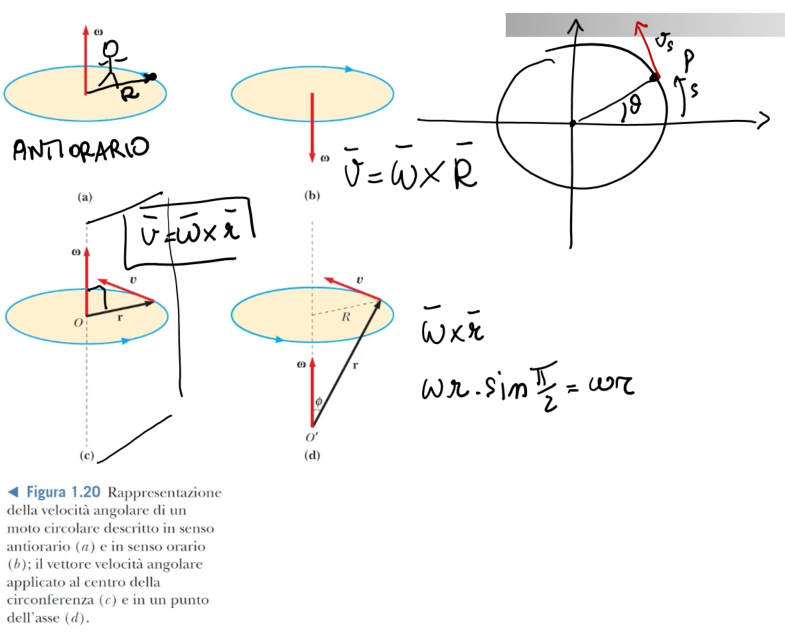
\includegraphics[width=0.5\textwidth]{moto_circolare2.png}
\end{figure}
\[
    v_s = \omega R
\]
\[
    \bar{v} = v_s \cdot \bar{u}_t
\]
\[
    \bar a = \dfrac{d\bar v}{dt} = \dfrac{\bar\omega\times\bar r}{dt} = \dfrac{d\bar \omega}{dt}\times\bar r + \bar\omega\times\dfrac{d\bar r}{dt}
\]
$wr\cdot\sin\frac{\pi}{2} = wr \ \ \ \bar\alpha = \dfrac{d\bar\omega}{dt} \ \ \ \bar a = \bar\alpha\times\bar r + \bar\omega\times\bar v \implies \bar a = \alpha\cdot r + \bar\omega\times\bar v$
\[
    \bar a_t = \bar\alpha\times\bar r
\]
\[
    \bar a_n = \bar{\omega}\times\bar v \ \ \ \textit{accelerazione centripeta}
\]
\end{document}